\documentclass[12pt]{article}

\usepackage{sbc-template}

%Image-related packages
\usepackage{graphicx}
\usepackage{subcaption}
\usepackage[utf8]{inputenc}
\usepackage[export]{adjustbox}
\usepackage{wrapfig}
%------------------------------
\usepackage[brazil]{babel}   
%\usepackage[latin1]{inputenc}  
\usepackage[utf8]{inputenc}  
% UTF-8 encoding is recommended by ShareLaTex
\usepackage{graphicx}
     
\sloppy
\title{Avaliação de Interface do Jogo Tower Siege}

\author{Ariel R. Nessi\inst{1}, Cristian Cotrena\inst{1}, Matheus S. Redecker\inst{1} }


\address{Pontifícia Universidade Católica do Rio Grande do Sul - PUCRS}

\begin{document} 

\maketitle

\begin{resumo} 
  A quantidade de jogos disponíveis na internet é vasta, este trabalho procura fazer uma avaliação crítica do jogo Tower Siege através de instrumento de avaliação de usabilidade. Este tipo de avaliação é vital para garantir a coesão geral do jogo, analisando da interface do jogo até quesitos de equilíbrio e satisfação do usuário. Este exercício visa preparar os membros para avaliar futuros projetos bem como desenvolver uma visão crítica sobre diversas dimensões de sistemas.
\end{resumo}


\section{Descrição do Sistema}

O sistema avaliado é o jogo Tower Siege, se trata de um jogo online, com opção de jogo singleplayer. O jogo é mistura conceitos de Tower Siege, que geralmente envolvem defender um objeto de invasores com conceitos de quebra-cabeça existentes em jogos como Candy Crush. Inicialmente o jogo demonstra um painel com opções para jogar, ver os créditos e indicações de outros jogos da produtora junto com um link para incorporar o jogo à um site(Figura ~\ref{fig:menuprincipal}).\\
Todos itens funcionais no menu esboçam alguma animação ao passar o mouse sobre estes, ao selecionar a opção "play" o usuario é transportado à uma nova tela onde está desenhado um mapa onde as 11 fases são representadas por torres. Cada torre possui estrelas, que indicam a performance do usuário nesta fase, caso a tenha jogado(Figura ~\ref{fig:mapainicial}).
No inicio do jogo apenas o primeiro nível é desbloqueado, o jogador precisa vencer para poder jogar nos níveis consequentes. 
Esta tela centraliza a navegação entre níveis, isto é, o jogador retorna a ela toda vez que finaliza uma fase. 
O jogador pode entre um nível e outro, 
navegar pela opção "upgrades" onde é possível comprar melhorias, com moedas de ouro. 
Existem 3 tipos de melhorias cada uma afeta uma mecânica diferente de jogo (Figura ~\ref{fig:upgrades}).
Ao clicar em uma torre o usuário pode escolher a dificuldade em que deseja jogar este nível e deve escolher entre "easy","medium" e "hard" (Figura ~\ref{fig:comecodificuldades}).
Os níveis consistem visualmente de dois blocos dividindo a tela, à esquerda está uma torre com blocos coloridos no meio, onde o jogador deve encontrar blocos da mesma cor para ganhar ouro e derrubar inimigos que tentam subir a torre. Na direita se encontra um painel onde é possível comprar reforços, armadilhas e magias para defender a torre, unidades são colocadas no topo da torre e cada uma possui uma mecânica de ataque diferente, variando poder e versatilidade da unidade.

\begin{figure}[h]
\begin{subfigure}{0.5\textwidth}
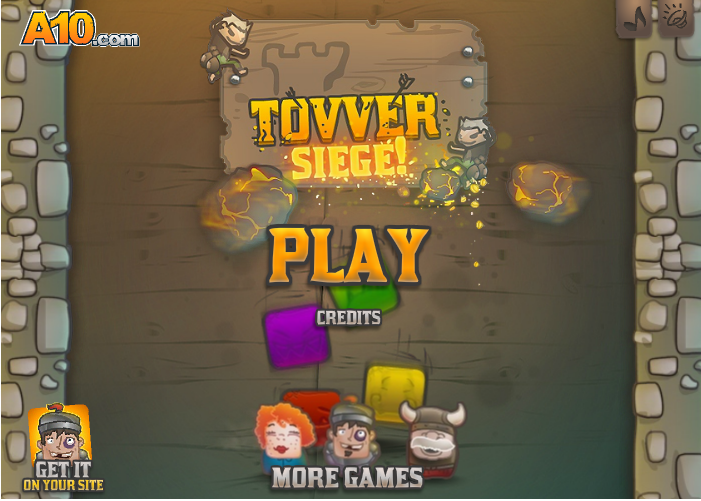
\includegraphics[scale=0.3]{imagens/menuprincipal.png}
\caption{Primeira tela do jogo}
\label{fig:menuprincipal}
\end{subfigure}
\begin{subfigure}{0.5\textwidth}
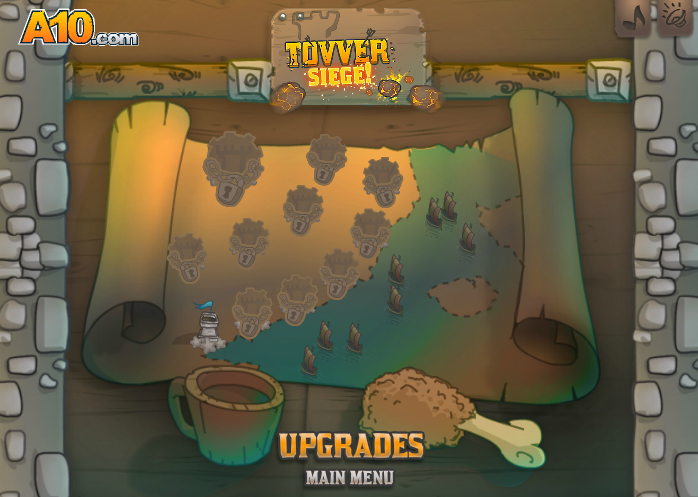
\includegraphics[scale=0.3]{imagens/mapainicial.png} 
\caption{Mapa Inicial do jogo}
\label{fig:mapainicial}
\end{subfigure}
\end{figure}

\begin{figure}[h]
\begin{subfigure}{0.5\textwidth}
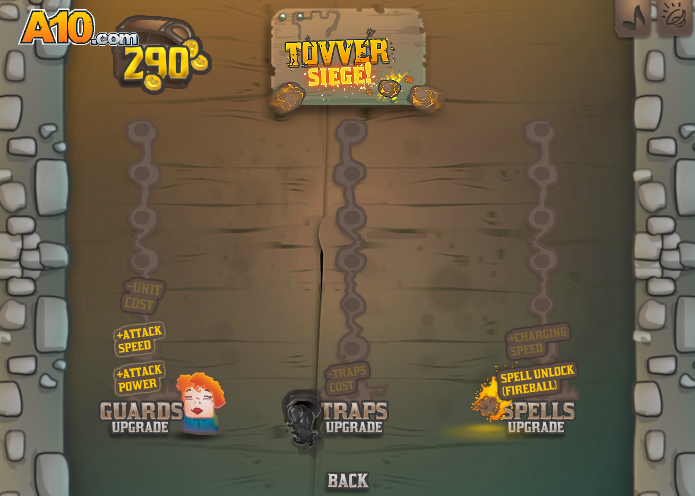
\includegraphics[scale=0.3]{imagens/upgrades.png}
\caption{Tela de upgrades}
\label{fig:upgrades}
\end{subfigure}
\begin{subfigure}{0.5\textwidth}
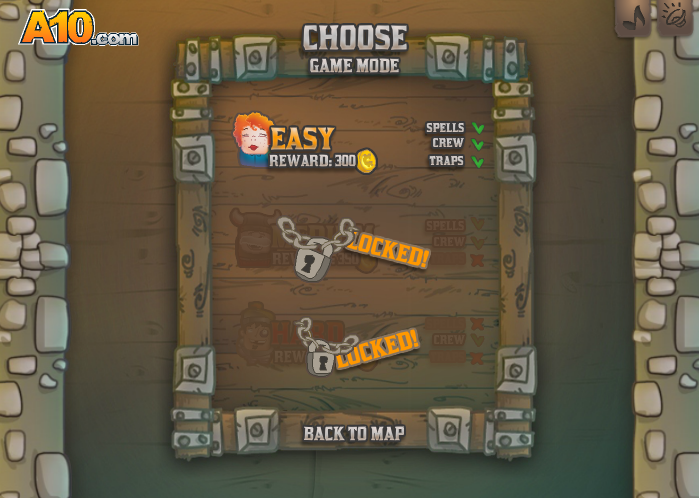
\includegraphics[scale=0.3]{imagens/comecodificuldades.png} 
\caption{Lista de dificuldades por nivel}
\label{fig:comecodificuldades}
\end{subfigure}
\end{figure}
\newpage
\section{Método de Avaliação}

    Inicialmente, adotamos uma avaliação por questionário, permitindo ao avaliador uma resposta de 1 a 5, significando 1 que discorda totalmente e 5 que concorda totalmente. Neste questionário, avaliamos os seguintes pontos:
        \begin{enumerate}
        \item Visibilidade do sistema;
        \item Correspondência entre o sistema e o mundo real;
        \item Controle e liberdade do usuário;
        \item Consistência e padronização;
        \item Prevenção de erros;
        \item Reconhecimento em vez de memorização;
        \item Flexibilidade e eficiência de uso;
        \item Projeto estético e minimalista;
        \item Ajude os usuários a reconhecerem, diagnosticarem e se recuperarem de erros;
        \item Ajuda e documentação;
        \item Jogabilidade;
        \item Extras;
        \item Satisfação.
        \end{enumerate}
        
    \paragraph{}Obtemos neste questionário as informações que cada avaliador possui do jogo de forma individual e, com estes dados,  realizamos uma avaliação heurística discutindo sobre as opiniões divergentes entre os avaliadores, formando assim, um relatório de avaliação.
   \paragraph{}As avaliações individuais apresentaram uma mesma percepção dos pontos fortes e fracos do jogo de maneira geral. As maiores divergências dentro das avaliações se deram nos tópicos 4,6 e 8, pois como são os tópicos que mais refletem no conceito de jogabilidade individual de cada um, em geral a opinião do grupo no que diz respeito ao sistema em si foi convergente.
   \paragraph{}O grupo definiu que o sistema apresenta um jogo que poderia ter sido muito melhor explorado e que não se tem vontade de continuar jogando e o grupo apresentou um conjunto de melhorias dentro do jogo que poderiam ser implementadas para que o mesmo seja mais interessante melhoria da historia do jogo, criação de um modo multiplayer, diferentes modos de jogo offline.


\section{Defeitos no Sistema}

\paragraph{} Ao analisarmos os dados que cada avaliador coletou sobre o jogo, percebemos vários pontos a serem melhorados e otimizados.\\
O jogo não possui uma opção "Fullscreen", sendo assim, usuários com dificuldades de visão terão problemas para utiliza-lo. \\
Também percebemos a existência de um leve "Delay" entre uma jogada e outra, impossibilitando assim o usuário em fazer jogadas de forma continua. \\
Durante uma partida, o jogo mostra algumas opções, dentre elas, existem as opções de "Menu" e "Pause". Estas duas opções realizam a mesma função que é pausar o jogo, porém, nesta pausa, o jogo mostra um ícone para o usuário ter acesso ao "Menu" do jogo, porém, o usuário só consegue entrar no menu se sair da partida. Como o sistema informa isto ao usuário, não seria de fato uma falha de navegação, mas podemos considerar este ponto como uma falha de usabilidade(Figura ~\ref{fig:menuerro}).
\paragraph{} Do início ao fim do jogo, a maioria dos icones possuem uma animação, porém, existem dois ícones que não possuem animações, um na tela inicial chamado "Get it On Your Site" e outro que aparece em todo momento chamado "A10.com", ambos estes ícones são links para outra página e aparentemente não possuem uma animação justamente para indicar isto, contudo, o botão "More Games" é um link e possui uma animação, quebrando assim o padrão (Figura ~\ref{fig:menuprincipal}).
\paragraph{} Para atingir os objetivos no jogo, o usuário precisa quebrar uma sequência de 3 blocos ou mais para ganhar dinheiro, porém, existem blocos especiais que podem ser quebrados individualmente e que quebram junto toda linha, após um tempo do começo do jogo tropas adversarias começam a escalar o jogo em busca de chegar ao topo para destruir a sua muralha, para evitar que isso aconteça existe também um espaço reservado na parte superior para alocação de tropas que podem ser adquiridas com o dinheiro conquistado quebrando blocos, e ainda na parte inferior existem espaços referentes a armadilhas para que antes de escalar os adversários sejam derrotados. Assim tudo parece muito legal, mas não é o que acontece na realidade, o jogo se torna muito previsível e cansativo, o jogador não se sente desafiado em nenhum momento e o jogo se torna repetitivo rapidamente.
\paragraph{} Temos uma série de tutoriais que são disponibilizados ao longo da primeira fase para o usuario que são bem fracos em questão de chamar o jogador para o jogo, são diretos e poderia ser apresentado de outra uma forma que o jogador se sentisse mais util e inteligente. No começo do jogo temos a tela que fala sobre a quebra dos blocos (Figura ~\ref{fig:tutorialblocos}), em seguida a tela que nos mostra nosso dinheiro(Figura ~\ref{fig:tutorialdinheiro}), e quando os inimigos começam a aparecer é apresentado a tela informando o que são e como derrotá-los(Figura ~\ref{fig:tutorialoquefazer}), a ultima é apresentado a tela de tutorial informando os soldados disponíveis e onde colocá-los (Figura ~\ref{fig:tutorialsoldado})

\begin{figure}[h]
\begin{subfigure}{0.5\textwidth}
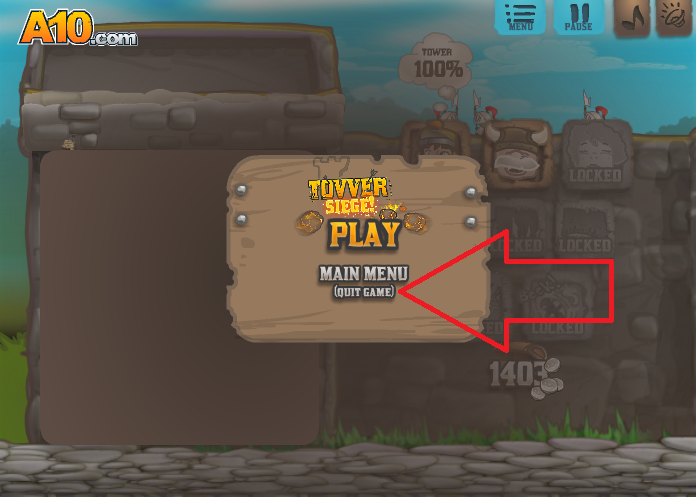
\includegraphics[scale=0.3]{imagens/menuerro.png}
\caption{Erro do menu}
\label{fig:menuerro}
\end{subfigure}
\begin{subfigure}{0.5\textwidth}
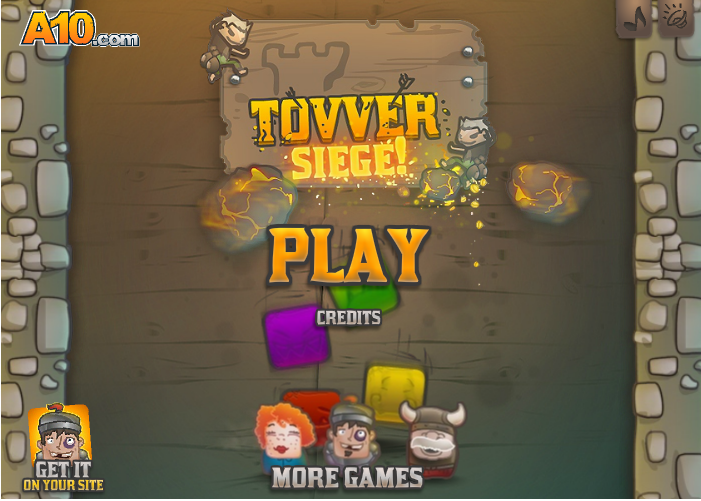
\includegraphics[scale=0.3]{imagens/menuprincipal.png} 
\caption{Menu principal com os icones descritos}
\label{fig:menuprincipal}
\end{subfigure}
\end{figure}

\begin{figure}[h]
\begin{subfigure}{0.5\textwidth}
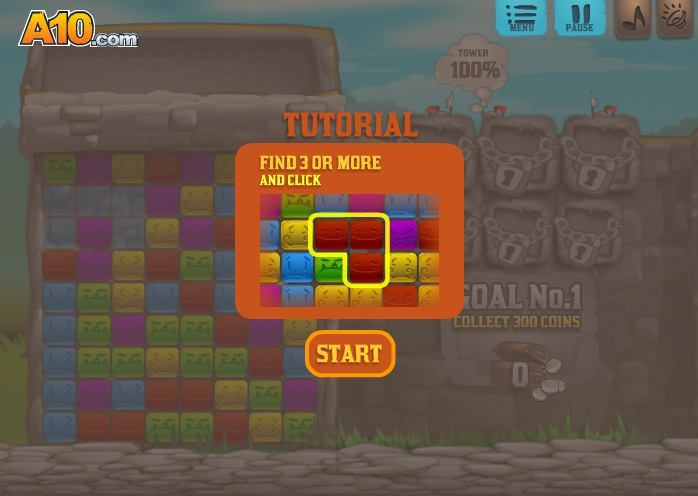
\includegraphics[scale=0.3]{imagens/tutorialblocos.png}
\caption{Tutorial blocos}
\label{fig:tutorialblocos}
\end{subfigure}
\begin{subfigure}{0.5\textwidth}
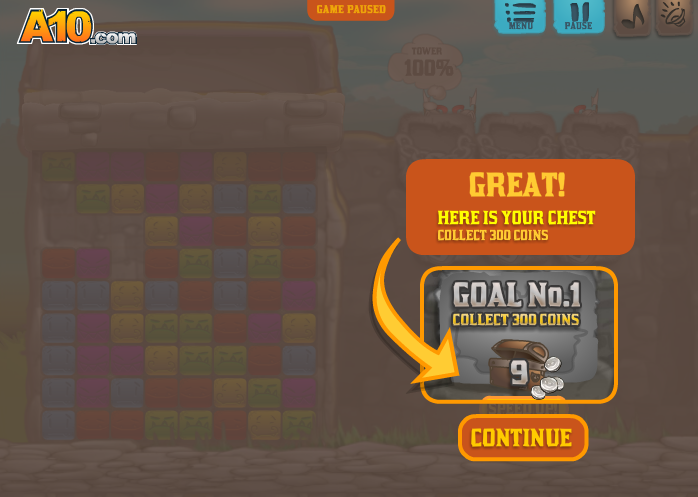
\includegraphics[scale=0.3]{imagens/tutorialdinheiro.png} 
\caption{Tutorial dinheiro}
\label{fig:tutorialdinheiro}
\end{subfigure}
\end{figure}

\begin{figure}[h]
\begin{subfigure}{0.5\textwidth}
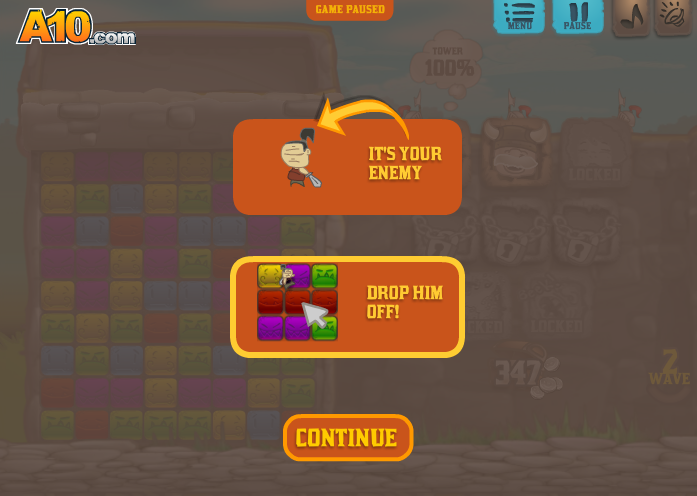
\includegraphics[scale=0.3]{imagens/tutorialoquefazer.png}
\caption{Tutorial como derrotar os inimigos}
\label{fig:tutorialoquefazer}
\end{subfigure}
\begin{subfigure}{0.5\textwidth}
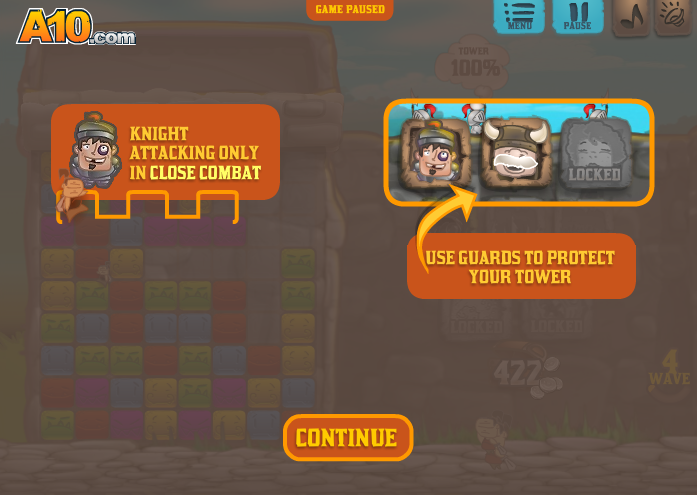
\includegraphics[scale=0.3]{imagens/tutorialsoldado.png} 
\caption{Tutorial das tropas}
\label{fig:tutorialsoldado}
\end{subfigure}
\end{figure}

\section{Conclusão}

\paragraph{} O jogo não atendeu as expectativas esperadas pelos usuários, pois não despertou curiosidade ou prazer ao decorrer das fases desmotivando assim o usuário a continuar no jogo após um período de tempo jogado.  \\
    
\paragraph{} Com base nas avaliações feitas, podemos concluir que o jogo apresentou muitas falhas que, se forem corrigidas deixarão o jogo muito mais interativo com o usuário e entre usuários.

\section{Referências}

A10.com. (30 de maio de 2015). Click Jogos. Fonte: http://www.clickjogos.com.br/jogos/tower-siege/

King.com. (30 de maio de 2015). Candy Crush Saga. Fonte: http://candycrushsaga.com/

\end{document}
